\documentclass[conference]{IEEEtran}
\usepackage{amsmath,amssymb}
\usepackage{graphicx}
\usepackage{booktabs}
\usepackage{url}
\usepackage{cite}
\usepackage{float}
\usepackage{array}
\graphicspath{{outputs/mobility_20261104_235027/figures/}}
\begin{document}
\title{Investigation of Sionna RT for Ray-Traced ISAC-Based Sensing}
\author{\IEEEauthorblockA{Indian Institute of Information Technology Vadodara, India\\[5pt]
\begin{tabular}{c@{\hspace{12mm}}c}
\textbf{Nandish Chauhan} & \textbf{Aahan Poddar} \\
202451040@iiitvadodara.ac.in & 202451184@iiitvadodara.ac.in \\
\end{tabular}\\[7pt]
\textit{Under the guidance of}\\[3pt]
\textbf{Dr. Bhupendra Kumar}\\
bhupendra\_kumar@iiitvadodara.ac.in}}
\maketitle
\begin{abstract}
Integrated sensing and communication (ISAC) motivates the study of radio channels that carry information about both communication links and the surrounding environment. This report investigates Sionna RT as a ray-tracing tool for generating geometrically interpretable propagation data in a three-dimensional scene. A fixed 3.5-GHz transmitter and a mobile receiver are placed in an exported urban-like environment; propagation paths are recomputed at 61 positions along a 1.183-km waypoint route. The saved balanced-profile run contains 4,826 valid path records and provides complex coefficients, delays, Doppler shifts, angles, interaction types, and surface geometry. Its coherent received power ranges from $-70.92$ to $-13.87$ dBm. Direct line of sight is present in 39 snapshots and absent in 22; every snapshot has at least one valid traced path. We describe the simulation, channel metrics, observed behavior, and the use of these outputs as inputs for subsequent sensing studies. The implemented work ends at ray tracing and channel analysis: no sensing waveform, target detector, estimator, or sensing accuracy evaluation is implemented.
\end{abstract}
\begin{IEEEkeywords}
Sionna RT, ray tracing, integrated sensing and communication, radio propagation, mobility, multipath, channel impulse response.
\end{IEEEkeywords}

\section{Introduction}
Wireless signals interact with their environment through propagation mechanisms such as reflection, transmission, and diffraction. These interactions affect communication quality but also contain information about the geometry and motion of objects. ISAC aims to exploit radio resources for both communication and sensing, creating an interest in channel models that expose path delays, angles, Doppler shifts, and interaction locations in addition to aggregate received power~\cite{liu2022}. Ray tracing offers one approach: a scene and radio-material model are used to predict propagation paths and their channel contributions.

This project investigates Sionna RT~\cite{sionna2025,sionna2023} as a tool to produce such data. The completed implementation considers a fixed transmitter and a receiver moving through a static three-dimensional environment. At each sampled receiver position, the notebook retraces multipath propagation, computes channel metrics, and stores both path-level and snapshot-level results. A separate radio map and visualizations help interpret spatial coverage and the modeled trajectory.

The scope is deliberately limited to the ray-tracing and analysis stage. The current scene does not contain a separately modeled sensing target or a monostatic radar return. No waveform, range--Doppler processing, target detection, localization algorithm, or experimental sensing validation is included. The report therefore treats sensing as a potential downstream application, not as a demonstrated result.

\section{Simulation Environment and Setup}
\subsection{Scene and Radio Configuration}
The scene is loaded from a Mitsuba XML file and three associated polygon meshes representing building geometry and a ground plane. The scene objects use ITU-style marble, metal, and concrete radio materials. Their saved material audit records a nominal thickness of 0.1 m and a scattering coefficient of zero for all three materials. These choices are modeling assumptions and are not field-calibrated measurements.

The transmitter is fixed at $(-107,43,10)$ m and operates at 3.5 GHz with 44 dBm configured transmit power and 20 MHz bandwidth. It uses a vertically polarized $4\times4$ planar array with half-wavelength element spacing and a 3GPP antenna pattern. The receiver is a vertically polarized single isotropic element at a height of 2 m. A synthetic-array configuration is used, and the channel is combined using equal-phase, equal-power transmitter weights. The 44 dBm value is the configured total input to this combining model, not a measured deployment power.

\begin{table}[t]
\caption{Parameters of the saved balanced-profile run}
\label{tab:setup}
\centering
\begin{tabular}{@{}ll@{}}\toprule
Parameter & Value \\ \midrule
Carrier frequency; bandwidth & 3.5 GHz; 20 MHz \\
Transmit power & 44 dBm \\
TX array; RX array & $4\times4$; $1\times1$ \\
TX position & $(-107,43,10)$ m \\
RX height; nominal speed & 2 m; 10 m/s \\
Waypoint arc length; duration & 1183.45 m; 118.35 s \\
Snapshots; path-solver depth & 61; 3 \\
Path samples per source & 100,000 \\
Radio map & $400\times400$ m, 4-m cells \\
Radio-map samples per TX & 250,000 \\
Random seed; synthetic array & 42; enabled \\
\bottomrule\end{tabular}
\end{table}

\begin{figure}[t]
\centering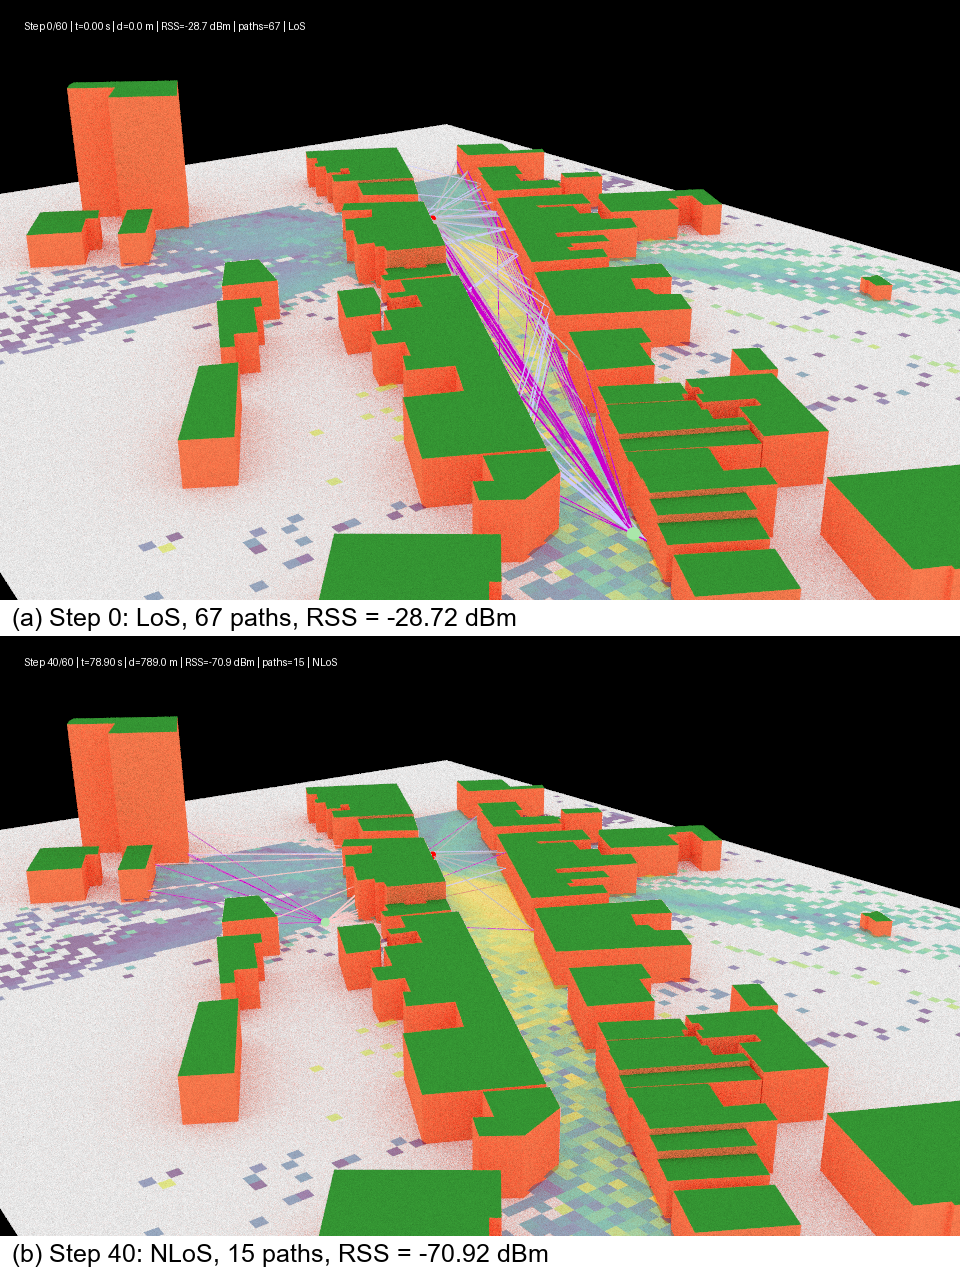
\includegraphics[width=0.95\columnwidth]{scene_los_nlos_comparison.png}
\caption{Saved scene renders at two sampled positions. The translucent radio map is a static overlay; the paths are retraced for each snapshot. Step 40 is the weakest coherent-RSS snapshot in the saved run.}
\label{fig:scene}\end{figure}

\subsection{Trajectory and Snapshot Procedure}
The receiver follows a road-aware waypoint polyline that approaches the transmitter, visits northern and southern/western branches, and returns to its start at $(160,-74,2)$ m. The notebook interpolates 61 positions uniformly in waypoint arc length. At the nominal speed of 10 m/s, the route represents approximately 118.35 s, and consecutive snapshots are separated by about 19.72 m and 1.97 s in arc-length and nominal time, respectively. Table~\ref{tab:setup} summarizes the run.

At each position, the receiver velocity and orientation are updated, and \texttt{PathSolver} computes propagation paths independently. Line of sight (LoS), specular and diffuse reflection, refraction, diffraction, and edge diffraction are enabled. Since the material scattering coefficients are zero, the run has no diffuse-category path records. Refraction uses the solver's material model and should not be interpreted as a full volumetric model of building interiors. The path solver is deterministic with a fixed seed; nevertheless, this single configuration does not establish numerical convergence.

Figure~\ref{fig:scene} compares the rendered scene at the initial and weakest-RSS snapshots. The trajectory is sampled uniformly along a polyline, but the velocity used at each snapshot is computed from the straight chord to the next sampled point divided by elapsed time. A chord can shortcut a corner or a reversal; the resulting velocity magnitude can thus be lower than the nominal 10 m/s, with consequences for the reported Doppler. The saved speeds range from approximately 0.68 to 10 m/s. This is a discretization limitation rather than an acceleration model of a real vehicle.

\subsection{Static Radio Map}
In addition to the path calculations, a separate radio-map solver produces a $400\times400$ m map centered at $(0,0,1.5)$ m with 4-m cells. Figure~\ref{fig:coverage} overlays the route, waypoints, and transmitter on the saved map. The map is calculated for a measurement plane at 1.5 m, whereas the moving receiver is at 2 m. The map and the coherent point-channel RSS are different solver products, so a map pixel should not be treated as the exact snapshot RSS at the same horizontal coordinate~\cite{sionna2025}.

\begin{figure}[t]
\centering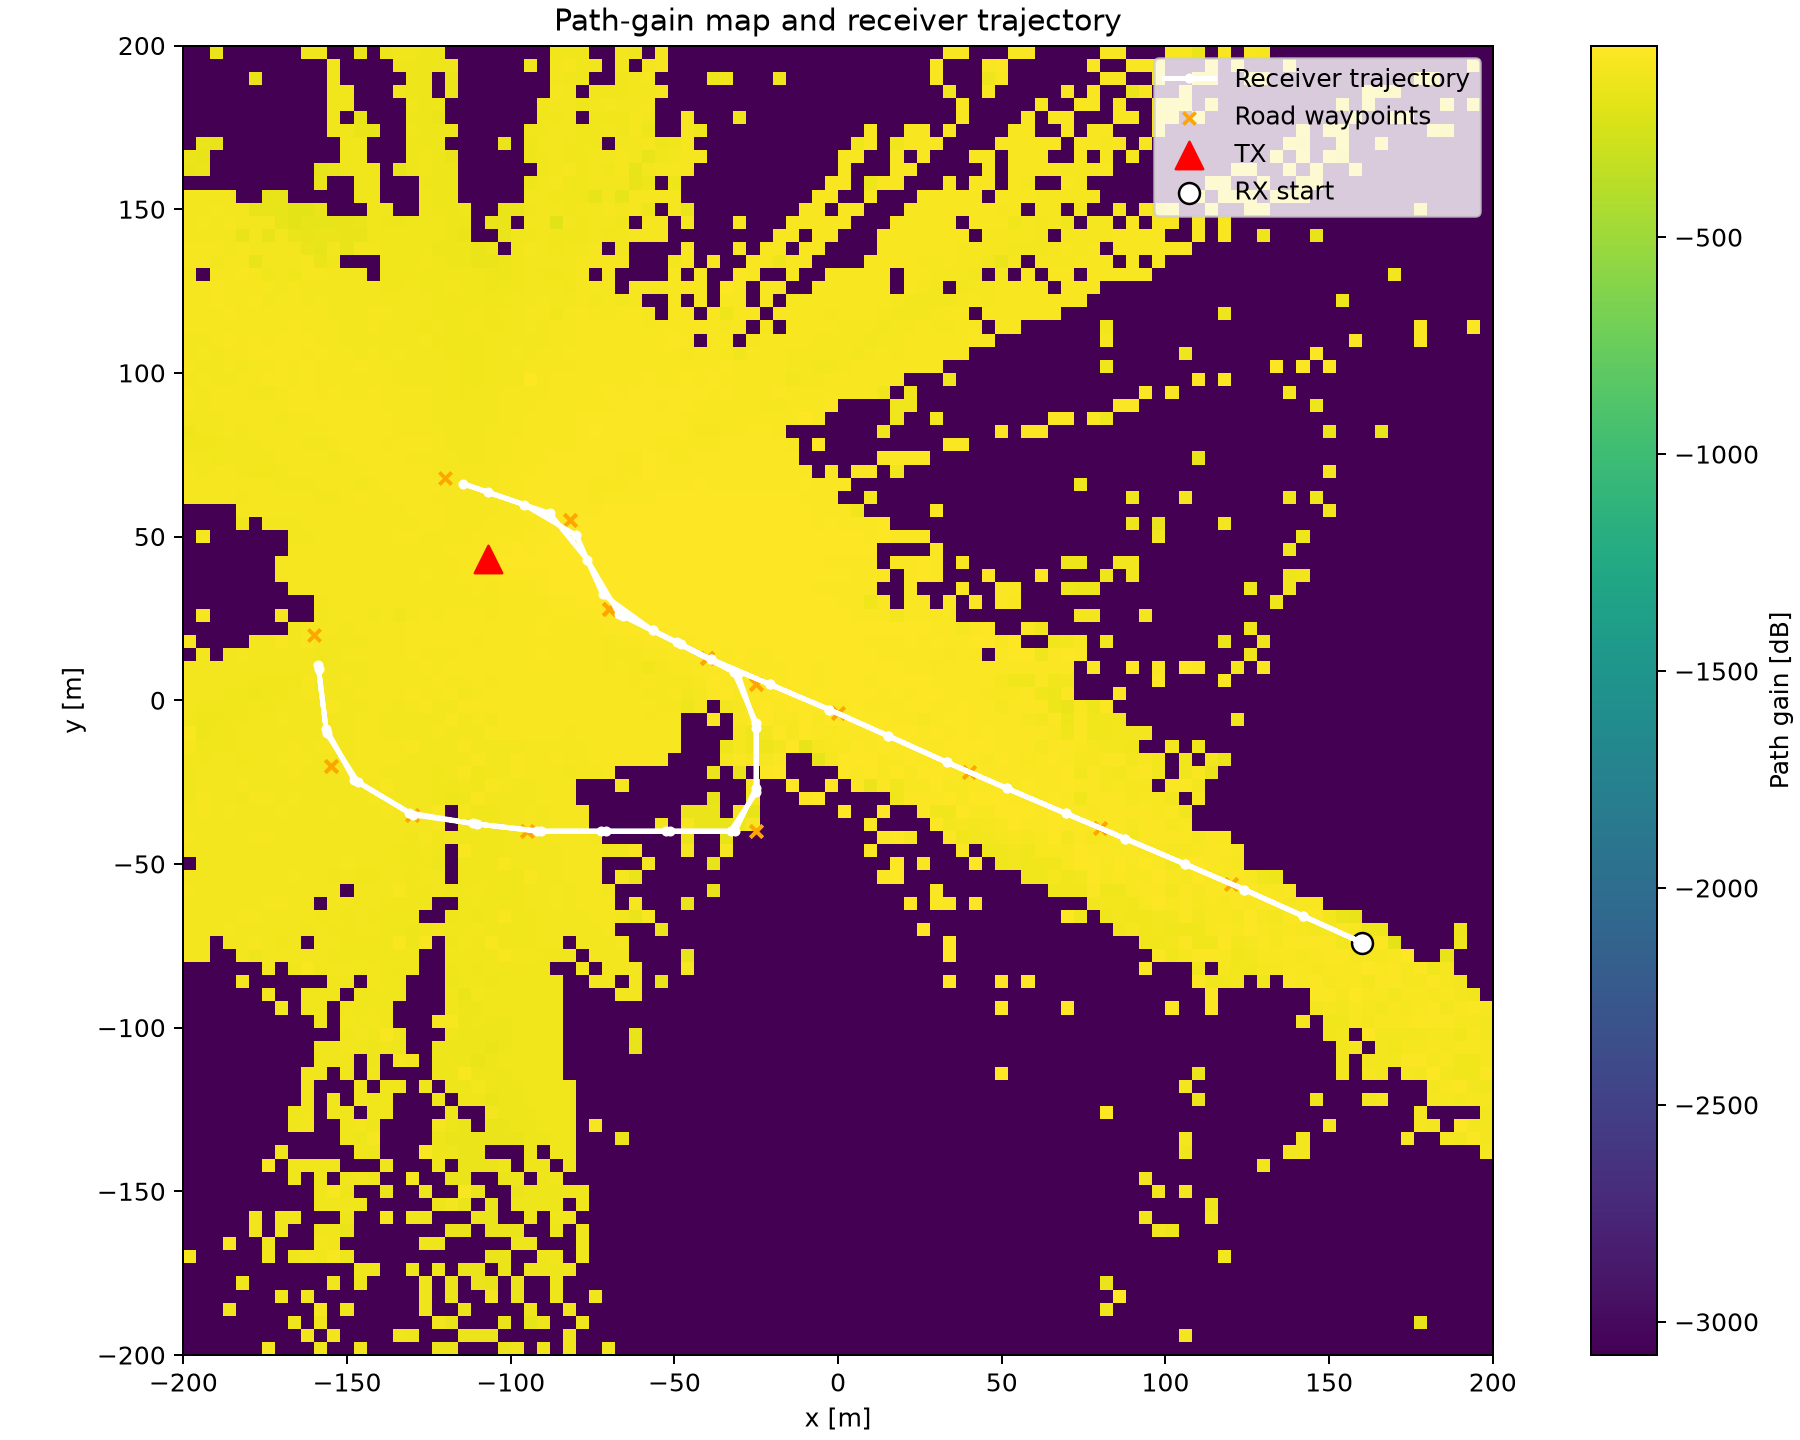
\includegraphics[width=\columnwidth]{coverage_and_trajectory.png}
\caption{Saved radio-map path gain and receiver trajectory. The map is evaluated at 1.5 m; the receiver trajectory is at 2 m.}
\label{fig:coverage}\end{figure}

\section{Channel Data and Metrics}
\subsection{Per-Path and Aggregate Channel}
For each snapshot, Sionna RT returns a complex coefficient $a_{m,i}$ for transmit antenna $m$ and path $i$, together with absolute path delay $\tau_i$, Doppler shift $f_{D,i}$, angles of departure and arrival, and interaction information. The notebook forms an effective coefficient with equal transmit weights:
\begin{equation}
h_i=\sum_{m=1}^{M} w_m a_{m,i},\qquad w_m=1/\sqrt{M},\quad M=16.
\label{eq:combine}
\end{equation}
For the valid paths at a snapshot, the reference-frequency narrowband complex channel is $H=\sum_i h_i$. The coherent received power and the incoherent sum used for comparison are
\begin{equation}
P_{\mathrm{coh}}=P_t\left|\sum_i h_i\right|^2,\qquad
P_{\mathrm{inc}}=P_t\sum_i |h_i|^2.
\label{eq:power}
\end{equation}
The coherent expression includes cross-path phase interference; the incoherent expression sums individual path powers. They serve different purposes, and their difference depends on the relative path phases. The quantity labeled RSS in this report is the notebook's coherent reference-frequency power, rather than a modeled wideband receiver measurement. The reported path loss is $-10\log_{10}|H|^2$ under the same antenna combining assumption.

The saved thermal-noise power is $8.09\times10^{-14}$ W ($-100.92$ dBm). The notebook divides coherent power by this quantity for an SNR estimate. This is a thermal-noise-only calculation: interference, receiver noise figure, implementation losses, receiver sensitivity, and bandwidth-dependent channel filtering are not modeled. Consequently, these SNR values do not demonstrate practical service performance.

\subsection{Delay, Doppler, and Path Classification}
For any per-path quantity $x_i$, the notebook uses $p_i=|h_i|^2$ as a weight, computes $\bar{x}=\sum_i p_i x_i/\sum_i p_i$, and defines its root-mean-square spread as
\begin{equation}
\sigma_x=\sqrt{\frac{\sum_i p_i(x_i-\bar{x})^2}{\sum_i p_i}}.
\label{eq:spread}
\end{equation}
Setting $x_i=\tau_i$ yields RMS delay spread; setting $x_i=f_{D,i}$ yields RMS Doppler spread. These are descriptive statistics of the resolved paths and should not be interpreted directly as ranging error or velocity-estimation accuracy.

Each valid path is assigned an exclusive category: direct LoS; specular, refraction, diffraction, or diffuse when its interactions are all of that type; or mixed when it contains multiple distinct interaction types. Counts are path records over snapshots, rather than unique physical paths or power fractions. Similarly, the sum of coherent group powers need not equal total coherent power because cross-terms between groups are omitted.

\section{Results and Discussion}
The following results use the saved run \texttt{mobility\_20261104\_235027}. Statistics are computed from its CSV files, not from older runs quoted in the project documentation. The 61 snapshots contain 4,826 valid path records, with between 12 and 133 valid paths per snapshot and a mean of 79.11. Table~\ref{tab:results} summarizes the principal results.

\begin{table}[t]
\caption{Summary of the saved simulation results}
\label{tab:results}\centering
\begin{tabular}{@{}ll@{}}\toprule
Metric & Result \\ \midrule
Valid path records & 4,826 \\
LoS / NLoS snapshots & 39 / 22 \\
Snapshots with no valid paths & 0 \\
Coherent RSS range & $-70.92$ to $-13.87$ dBm \\
Thermal-only SNR range & 30.00 to 87.05 dB \\
RMS delay spread range & 2.40 to 266.86 ns \\
RMS Doppler spread range & 0.39 to 55.21 Hz \\
Strongest RSS & step 19, 374.76 m \\
Weakest RSS & step 40, 788.97 m \\
\bottomrule\end{tabular}
\end{table}

\subsection{Line-of-Sight Transitions and Power}
The direct path is present initially, is absent from step 23 through step 44, and returns at step 45. These are transitions between sampled positions: the exact distances at which blockage starts or ends are not resolved by the simulation. All 22 NLoS snapshots still have valid multipath, so absence of LoS does not imply a ray-tracing outage. An actual service outage would require an explicit receiver performance or sensitivity threshold, neither of which is defined here.

The maximum coherent RSS is $-13.87$ dBm at step 19, with 125 valid paths and LoS. The minimum is $-70.92$ dBm at step 40, with 15 valid paths and no LoS. The spread between these extremes is approximately 57.05 dB. The result reflects geometry, antenna response, material assumptions, and phase interference; it should not be generalized to other urban scenes without further study. At the weakest snapshot the incoherent sum is $-63.26$ dBm, approximately 7.65 dB above the coherent value, illustrating destructive interference among the modeled paths.

Figure~\ref{fig:metrics} shows coherent and incoherent power, path loss, delay spread, Doppler spread, and path count over the route. Across this run, the coherent-minus-incoherent difference ranges from approximately $-10.88$ to $+5.87$ dB. Since the channel is evaluated at a reference frequency, small geometric or frequency changes can alter the phases and hence this difference.

\begin{figure}[t]
\centering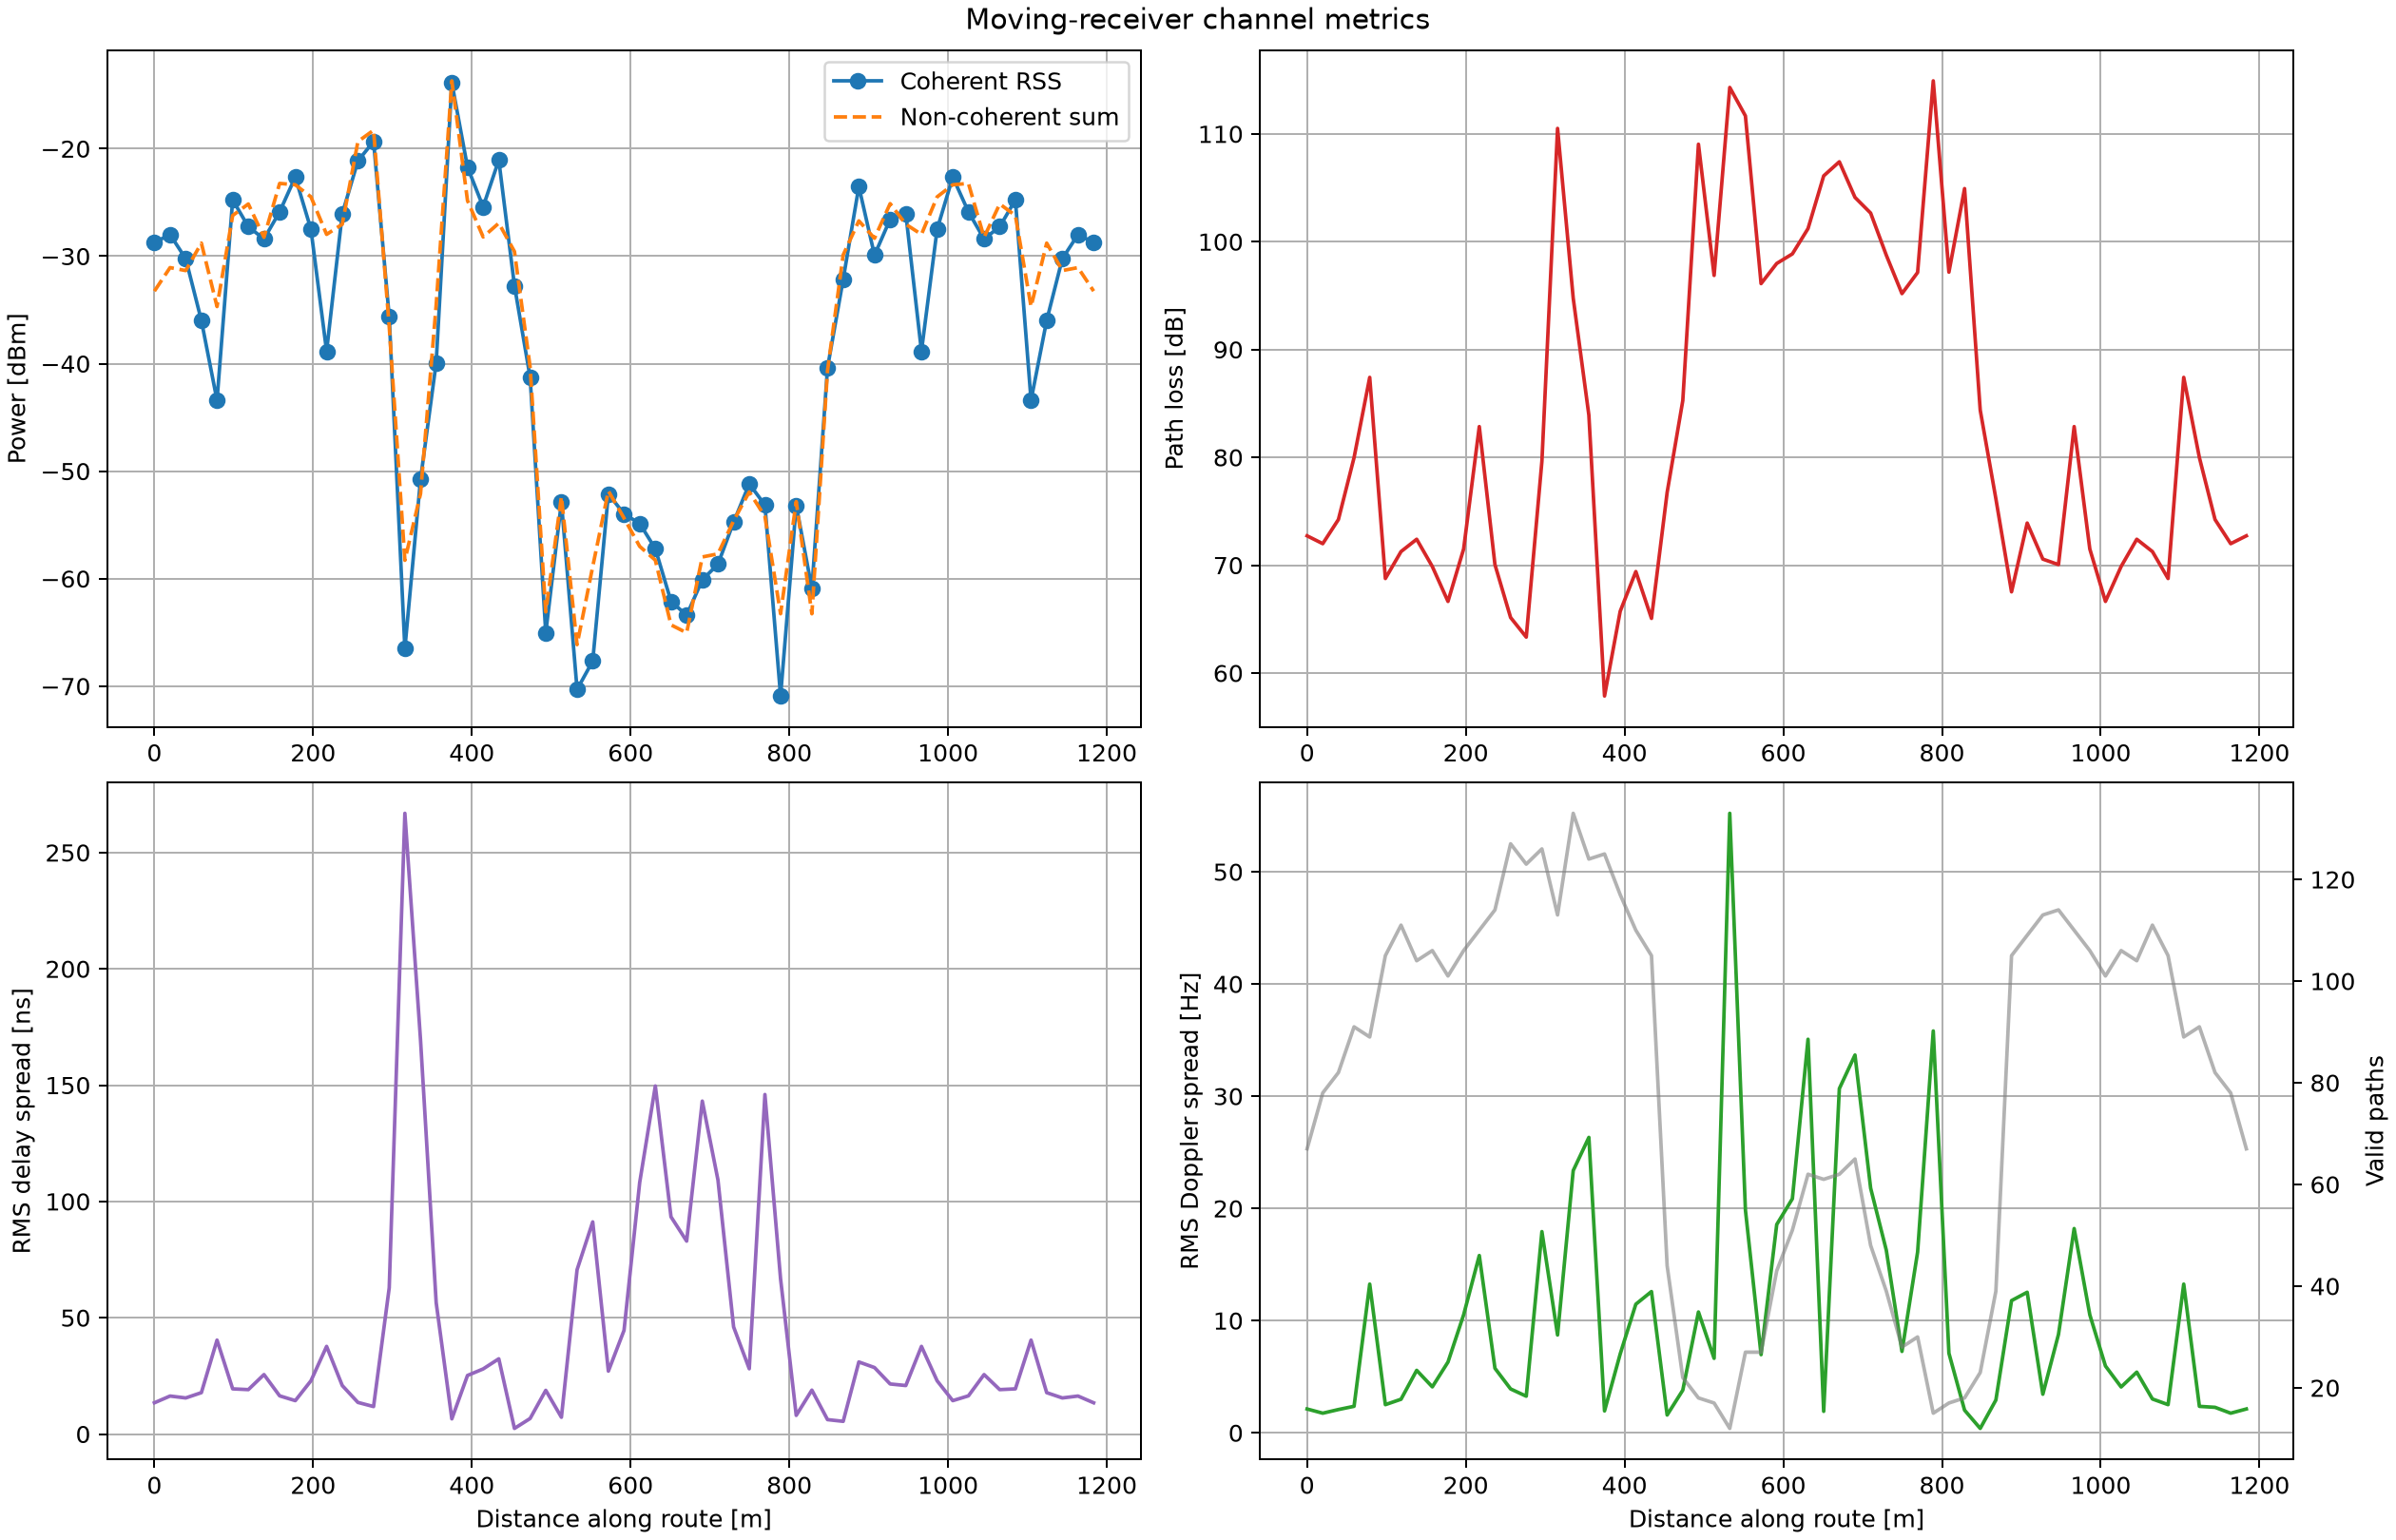
\includegraphics[width=\columnwidth]{channel_metrics.png}
\caption{Snapshot channel metrics along the receiver route. Coherent and incoherent powers differ because of multipath phase.}
\label{fig:metrics}\end{figure}

\begin{figure}[t]
\centering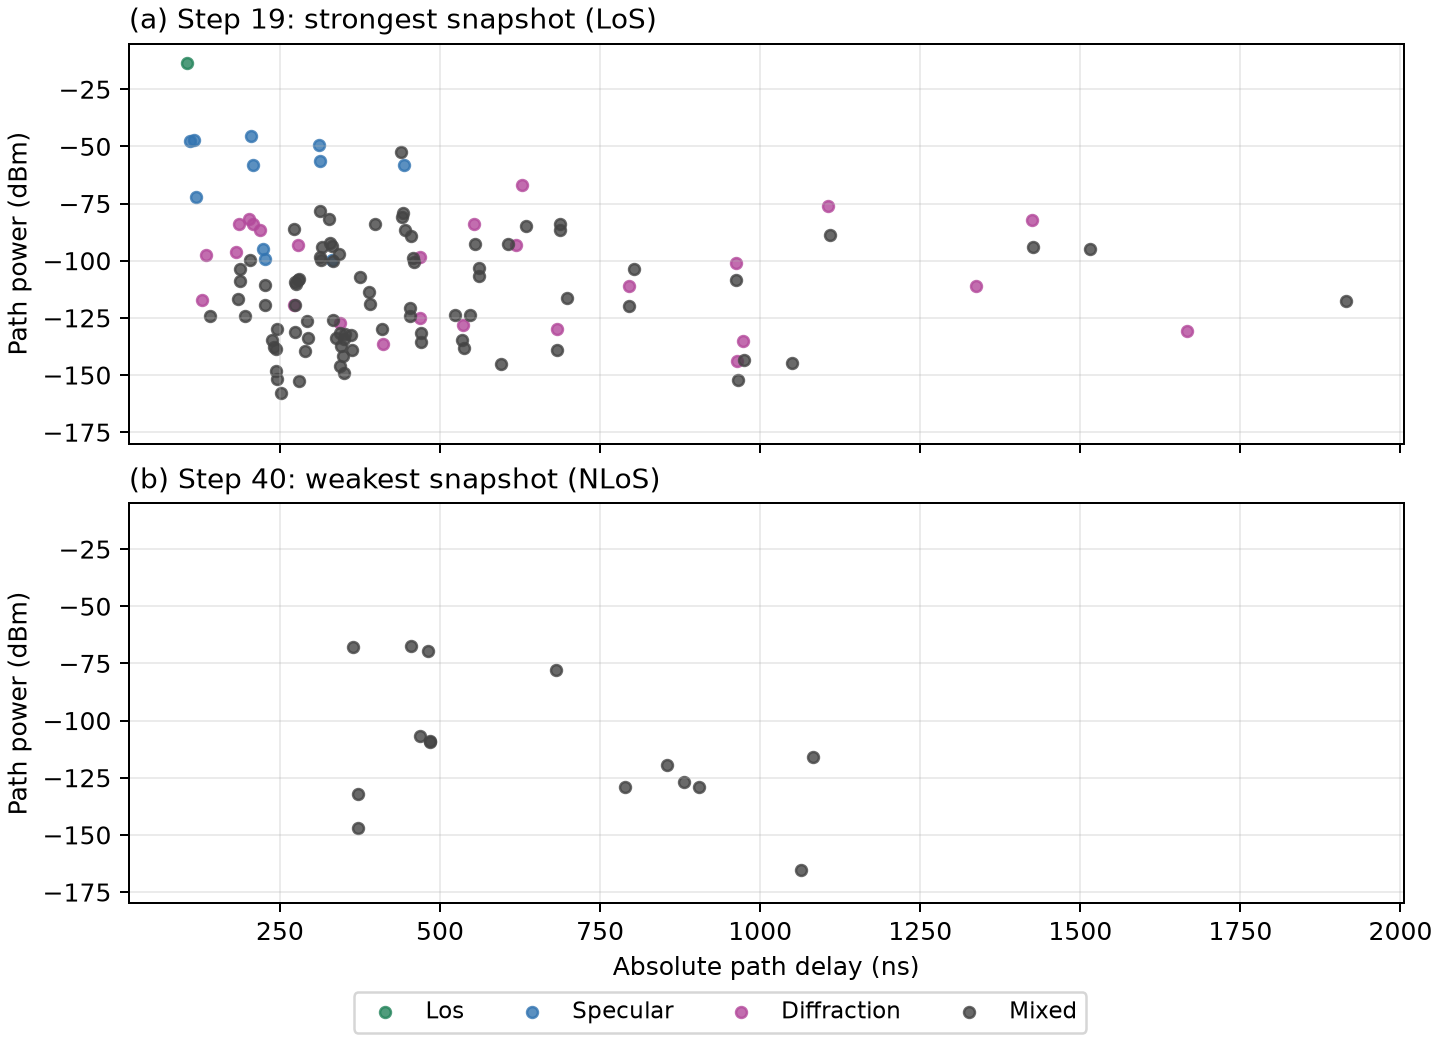
\includegraphics[width=\columnwidth]{strong_weak_path_delays.png}
\caption{Path powers and absolute delays for the strongest and weakest coherent-RSS snapshots. Each point represents one valid path; category colors follow the path interaction classification.}
\label{fig:delaycompare}\end{figure}

\subsection{Propagation Mechanisms}
The path records comprise 39 LoS, 337 specular-only, 14 refraction-only, 1,010 diffraction-only, and 3,426 mixed records; there are no diffuse-only records. Mixed interactions form the largest share by count, but this does not imply that they dominate received power. The category-level coherent powers in Fig.~\ref{fig:mechanisms} depend on phase and the number and strength of the paths in each group. The absence of diffuse-category records is consistent with the zero scattering coefficients in the material audit; it is not evidence that real surfaces have no diffuse scattering.

\begin{figure}[t]
\centering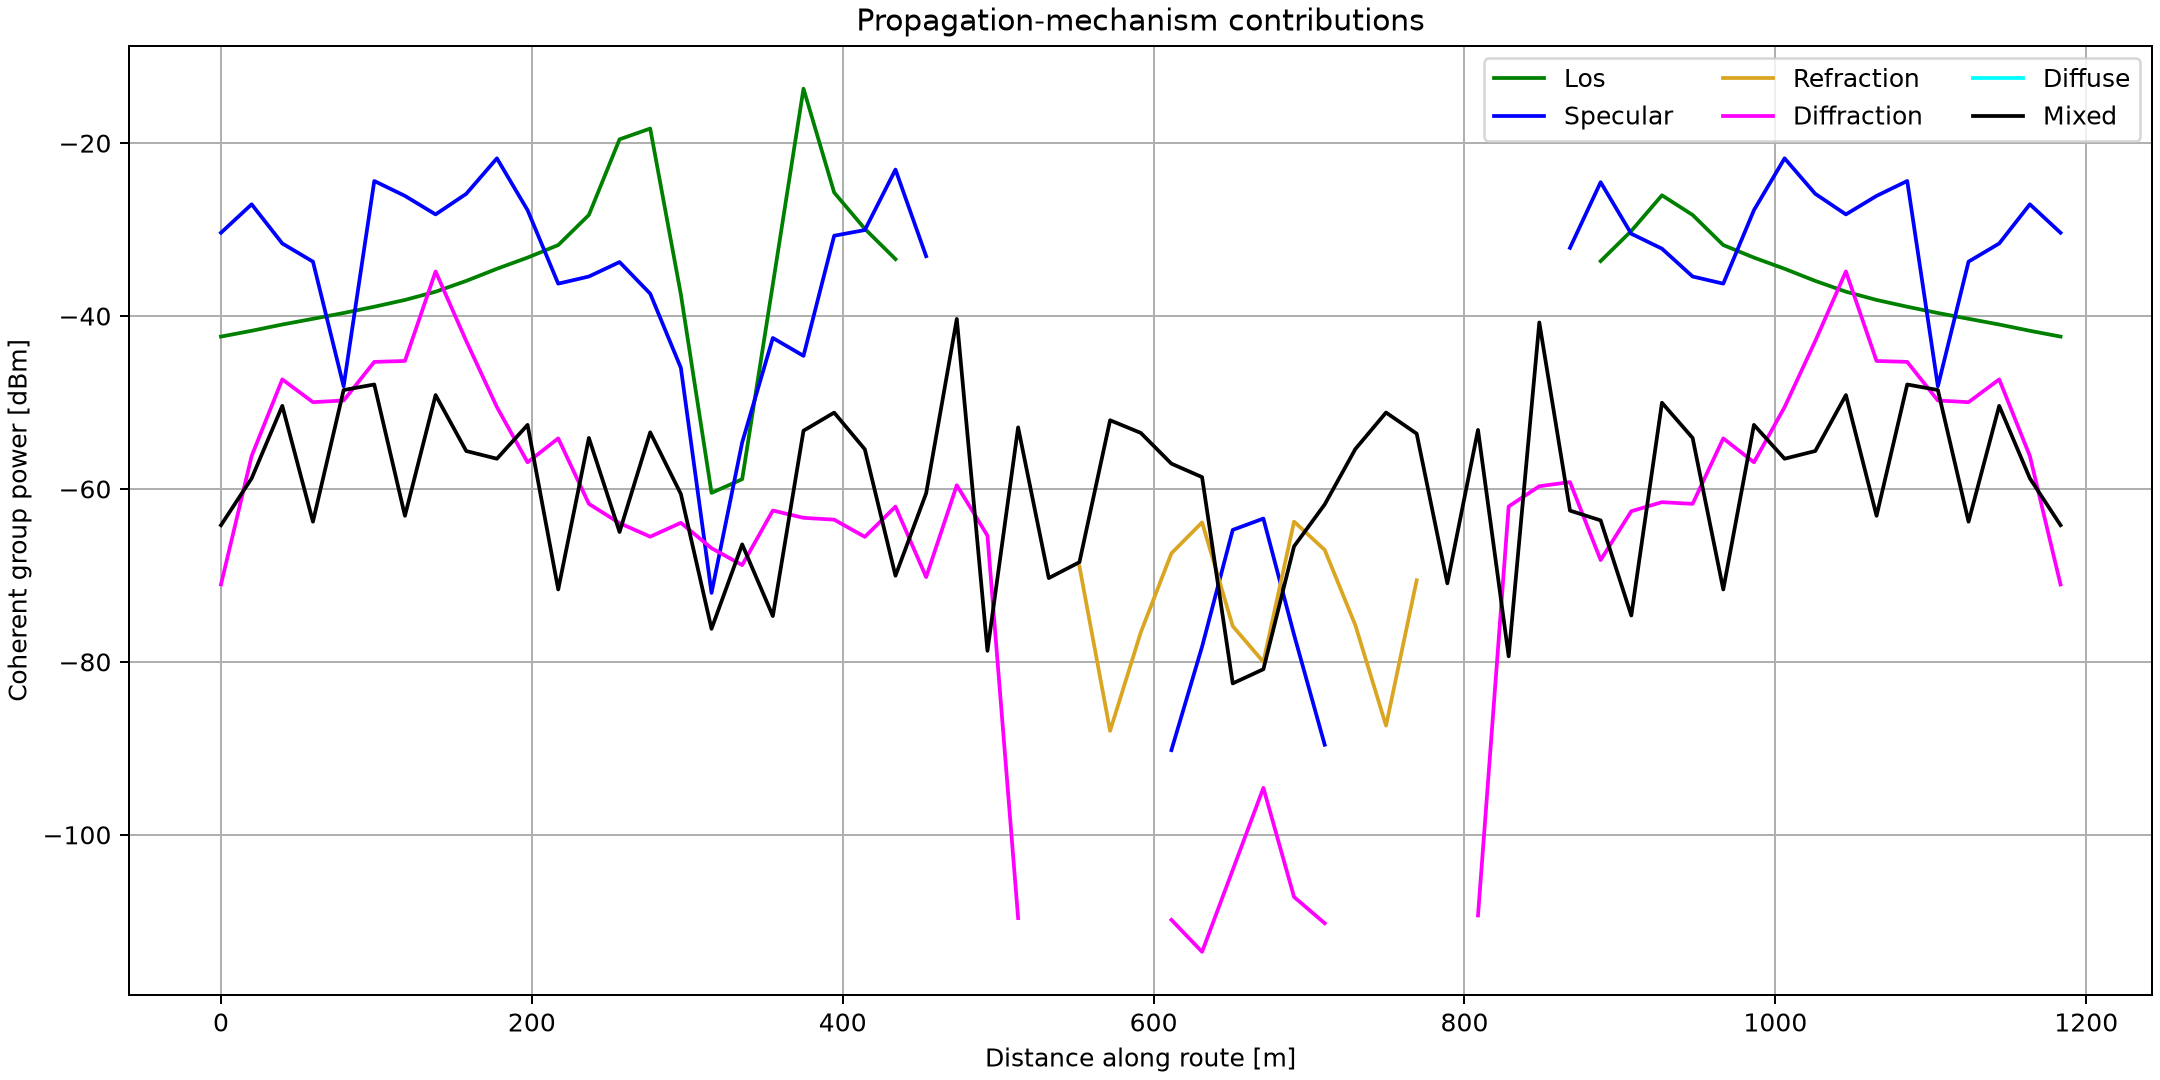
\includegraphics[width=\columnwidth]{mechanism_contributions.png}
\caption{Coherently summed power within each interaction category. Group powers are not additive because inter-group interference is excluded.}
\label{fig:mechanisms}\end{figure}

\subsection{Delay and Doppler Characteristics}
RMS delay spread varies from 2.40 to 266.86 ns across the snapshots, reflecting differences in the relative delays and strengths of modeled paths. The maximum RMS Doppler spread is 55.21 Hz. These results are sensitive to sampling, path discovery, weights, and the chord-derived receiver velocity. They are also different from the Doppler of any one path. For example, at the route's first and last snapshots the receiver position is the same and the coherent RSS is about $-28.72$ dBm, while the weighted mean Doppler changes sign from approximately $+113.10$ to $-113.10$ Hz as the travel direction reverses. This illustrates the motion information represented in the path output, subject to the stated velocity model.

Figure~\ref{fig:delaycompare} compares the path-delay distributions at the strongest and weakest snapshots; these path powers are individual contributions, not the coherently summed RSS. Figure~\ref{fig:pdp} shows the saved final snapshot's path geometry and power--delay profile. Its geometry panel depicts traced paths and the trajectory, rather than a full rendering of the buildings. Absolute delays and per-path powers allow individual contributions to be inspected, including paths weaker than the dominant component. Local path indices are assigned independently at each snapshot, so an identical index at different steps must not be assumed to identify the same physical path.

\begin{figure}[t]
\centering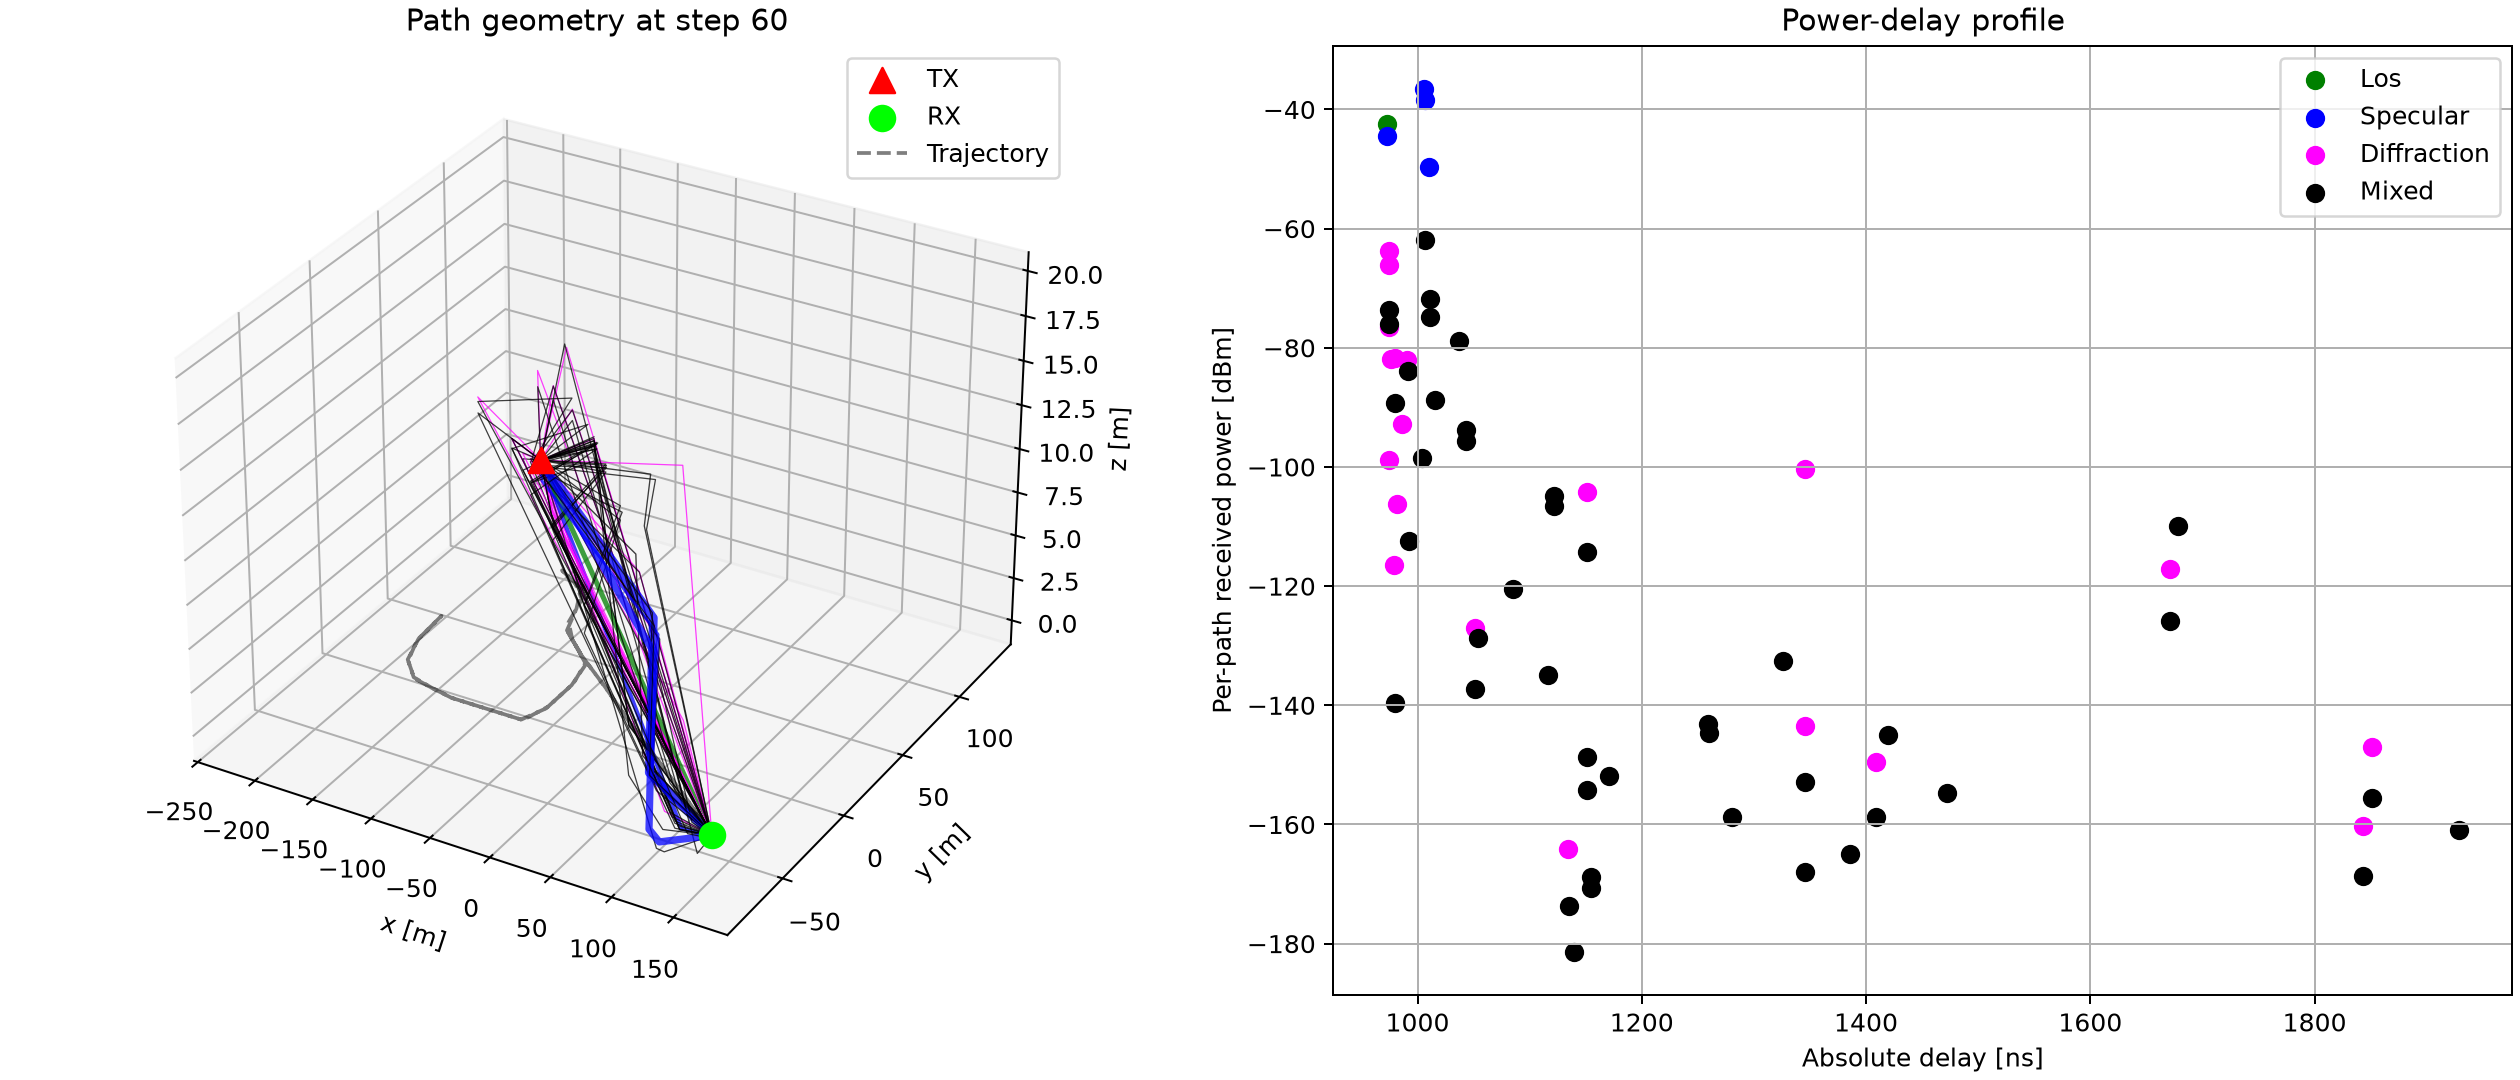
\includegraphics[width=\columnwidth]{snapshot_060_paths_and_pdp.png}
\caption{Final-snapshot ray geometry and path-level power--delay profile. Colors identify the notebook's interaction categories.}
\label{fig:pdp}\end{figure}

\section{Outputs and Potential ISAC Applications}
The completed workflow exports \texttt{path\_data.csv} with a record for each valid path, \texttt{snapshot\_summary.csv} with aggregate channel metrics, and \texttt{channel\_arrays.npz} with padded numerical arrays and a validity mask. The path records contain complex amplitudes, delays, Doppler shifts, departure and arrival angles, interaction sequences, object and material names, primitive IDs, and interaction vertices. The configuration JSON and material audit document key assumptions, while figures and a GIF provide visualization. The GIF shows selected discrete snapshots; it does not demonstrate continuous propagation or target tracking. The radio map is saved as visual output but its raw numerical cells are not exported.

These outputs offer several possible inputs to later communication and sensing investigations:
\begin{itemize}
\item \emph{Delay and range-related analysis:} path delays can support construction of a channel impulse response and investigation of path separability. A delay-to-range conversion must use the correct geometry: these are one-way transmitter--receiver propagation paths, not automatically monostatic round-trip target ranges.
\item \emph{Motion analysis:} per-path Doppler can be used to explore how relative motion influences observed frequency shifts. A sensing system would still need a waveform, coherent observation interval, and an estimator.
\item \emph{Angular and spatial analysis:} departure and arrival angles, surface IDs, and vertices can help relate path changes to scene geometry and investigate angular signatures or multipath-assisted localization.
\item \emph{Channel and waveform evaluation:} complex path coefficients and delays can be used as inputs to a frequency-selective channel model or a subsequent link-level simulation. The necessary bandwidth, filtering, and noise assumptions must be made explicit.
\item \emph{Environment-aware studies:} repeating the simulation with changed geometry, receiver motion, or calibrated materials could help study blockage, visibility, and the sensitivity of inferred features to scene changes.
\end{itemize}
These are prospective uses of ray-traced channel data. A dedicated sensing experiment would require a target and a suitable propagation configuration, such as an explicitly modeled transmitter--target--receiver geometry, together with a processing chain and a clearly defined evaluation metric.

\section{Limitations and Future Work}
The current results describe one simulated route in one static scene; they are not field measurements. The building meshes and ITU-style materials are approximations, and no measured scattering coefficients or material calibration are provided. Other vehicles, pedestrians, foliage, atmospheric effects, hardware losses, interference, and changing environmental geometry are absent. Solver sampling and interaction depth can miss weak paths; the balanced run has not been compared with higher-fidelity settings or measured data. The stored JSON also omits some provenance, including the solver seed and array geometry, which must be recovered from the notebook.

A natural next step is to compare snapshot spacing, path samples, and interaction depth to assess numerical sensitivity, and to refine trajectory velocity near turns. The next sensing stage could add a well-defined target and an appropriate bistatic or monostatic setup, generate channel responses over a specified waveform bandwidth and observation time, and implement range, Doppler, or angle estimation. Any such extension should compare the estimates with known scene ground truth and, where possible, measurements. Practical link analysis would additionally require receiver noise figure, interference and an explicit outage criterion.

\section{Conclusion}
This project established a reproducible ray-tracing and channel-analysis workflow using Sionna RT for a moving receiver in a static scene. In the saved 3.5-GHz experiment, the route produced 4,826 path records over 61 snapshots and exhibited a direct-path blockage and return, without a no-valid-path outage. The outputs describe multipath geometry, complex coefficients, delay, Doppler, and angles, making them useful foundations for subsequent ISAC experiments. The present results stop at simulated propagation and channel analysis; sensing performance remains to be implemented and validated.

\begin{thebibliography}{1}
\bibitem{liu2022} F. Liu \emph{et al.}, ``Integrated sensing and communications: Toward dual-functional wireless networks for 6G and beyond,'' \emph{IEEE J. Sel. Areas Commun.}, vol. 40, no. 6, pp. 1728--1767, 2022, doi: 10.1109/JSAC.2022.3156632.
\bibitem{sionna2025} F. A\"it Aoudia, J. Hoydis, M. Nimier-David, S. Cammerer, and A. Keller, ``Sionna RT: Technical report,'' arXiv:2504.21719, 2025. [Online]. Available: \url{https://arxiv.org/abs/2504.21719}
\bibitem{sionna2023} J. Hoydis \emph{et al.}, ``Sionna RT: Differentiable ray tracing for radio propagation modeling,'' arXiv:2303.11103, 2023. [Online]. Available: \url{https://arxiv.org/abs/2303.11103}
\end{thebibliography}
\end{document}
